\documentclass[11pt]{article}

\usepackage{amsmath,amssymb,mathtools}
\usepackage[margin=1in]{geometry}
\usepackage{hyperref}

\newcommand{\R}{\mathbb{R}}
\newcommand{\Sph}{\mathbb{S}}
\newcommand{\Id}{\mathrm{Id}}

\usepackage{tikz}
\usepackage{tikz-3dplot}
\usetikzlibrary{arrows.meta, calc, positioning}

\title{Shape Operator on $S^2$ in Spherical Coordinates $(\theta,\phi)$}
\author{}
\date{}

\begin{document}
	\maketitle
	
	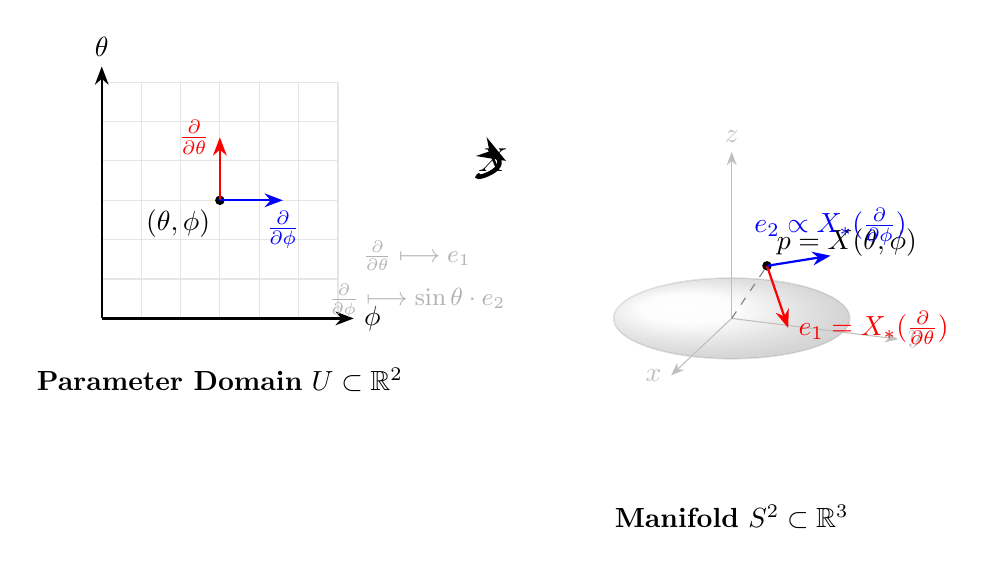
\begin{tikzpicture}[>=Stealth, node distance=2cm]
		
		% --- 1. THE DOMAIN (Parameter Space) ---
		\begin{scope}[local bounding box=Domain]
			% Draw the grid (Theta vertical, Phi horizontal for visualization)
			\draw[step=0.5, gray!20, thin] (0,0) grid (3,3);
			\draw[->, thick] (0,0) -- (3.2,0) node[right] {$\phi$};
			\draw[->, thick] (0,0) -- (0,3.2) node[above] {$\theta$};
			
			% The specific point (theta_0, phi_0)
			\coordinate (uv) at (1.5, 1.5);
			\filldraw (uv) circle (1.5pt) node[below left] {$(\theta, \phi)$};
			
			% The Domain Basis Vectors
			% d/dtheta (Vertical change in theta)
			\draw[red, thick, ->] (uv) -- ++(0, 0.8) node[left] {$\frac{\partial}{\partial \theta}$};
			
			% d/dphi (Horizontal change in phi)
			\draw[blue, thick, ->] (uv) -- ++(0.8, 0) node[below] {$\frac{\partial}{\partial \phi}$};
			
			% Label
			\node[anchor=north] at (1.5, -0.5) {\textbf{Parameter Domain} $U \subset \mathbb{R}^2$};
		\end{scope}
		
		
		% --- 2. THE CODOMAIN (Sphere S^2) ---
		\begin{scope}[xshift=8cm, scale=1.5]
			% Setup 3D view
			\tdplotsetmaincoords{70}{110}
			\begin{scope}[tdplot_main_coords]
				
				% Sphere
				\draw[gray!30] (0,0,0) circle (1);
				\draw[gray!20] (1,0,0) arc (0:360:1); % Equator
				\shade[ball color=gray!10, opacity=0.3] (0,0,0) circle (1);
				
				% Axes
				\draw[->, gray!50] (0,0,0) -- (1.5,0,0) node[left] {$x$};
				\draw[->, gray!50] (0,0,0) -- (0,1.5,0) node[right] {$y$};
				\draw[->, gray!50] (0,0,0) -- (0,0,1.5) node[above] {$z$};
				
				% The Point p = X(theta, phi)
				% Let's pick theta=45, phi=45
				\tdplotsetcoord{P}{1}{45}{45}
				\filldraw (P) circle (1.0pt) node[anchor=south west] {$p = X(\theta, \phi)$};
				\draw[dashed, gray] (0,0,0) -- (P);
				
				% The Pushed Forward Vectors
				
				% e1 = X_theta (Tangent to Meridian, South)
				% Calculation: (cos45cos45, cos45sin45, -sin45) = (0.5, 0.5, -0.707)
				\draw[red, thick, ->] (P) -- ++(0.3, 0.3, -0.42) node[right] {$e_1 = X_*(\frac{\partial}{\partial \theta})$};
				
				% e2 = X_phi (Tangent to Parallel, East)
				% Calculation: (-sin45, cos45, 0) = (-0.707, 0.707, 0)
				\draw[blue, thick, ->] (P) -- ++(-0.42, 0.42, 0) node[above] {$e_2 \propto X_*(\frac{\partial}{\partial \phi})$};
				
			\end{scope}
			
			% Label
			\node[anchor=north] at (0, -1.5) {\textbf{Manifold} $S^2 \subset \mathbb{R}^3$};
		\end{scope}
		
		
		% --- 3. THE MAPPING ARROW (The "To" / "Mapsto") ---
		
		% Draw a big curved arrow from domain to codomain
		\draw[->, ultra thick, shorten >= 1cm, shorten <= 1cm] 
		(Domain.east) to[out=30, in=150] node[midway, above, font=\large] {$X$} (6, 1.5);
		
		% Explicit "Mapsto" labels for the vectors
		\node[align=center, font=\small, gray!60] at (4, 0.5) {
			$\frac{\partial}{\partial \theta} \longmapsto e_1$ \\[0.5em]
			$\frac{\partial}{\partial \phi} \longmapsto \sin\theta \cdot e_2$
		};
		
	\end{tikzpicture}

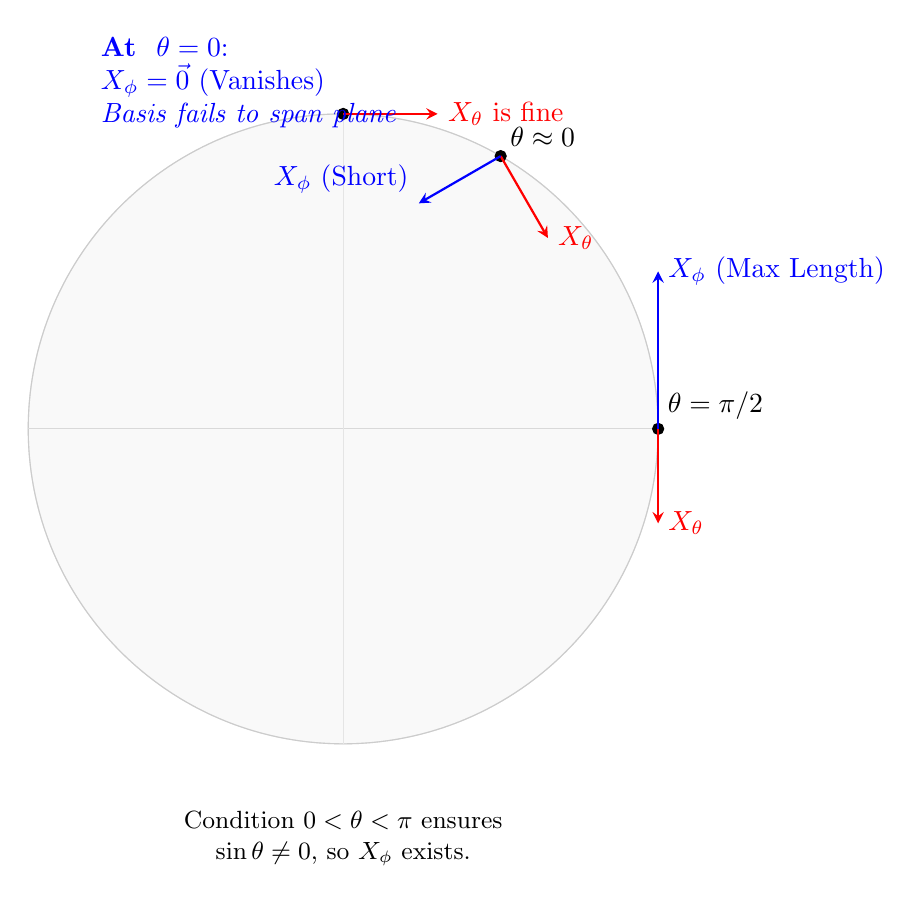
\begin{tikzpicture}[scale=4, >=stealth]
	
	% Sphere outline
	\draw[gray!20, fill=gray!5] (0,0) circle (1);
	\draw[gray!40] (0,0) circle (1);
	\draw[gray!30] (-1,0) -- (1,0); % Equator line
	\draw[gray!20] (0,-1) -- (0,1); % Axis
	
	% --- POINT 1: EQUATOR (Good Basis) ---
	\coordinate (P1) at (1,0);
	\filldraw (P1) circle (0.5pt);
	\draw[red, thick, ->] (P1) -- ++(0,-0.3) node[right] {$X_\theta$};
	\draw[blue, thick, ->] (P1) -- ++(0,0.5) node[right] {$X_\phi$ (Max Length)};
	\node[anchor=south west] at (P1) {$\theta=\pi/2$};
	
	% --- POINT 2: NEAR POLE (Weak Basis) ---
	\coordinate (P2) at (0.5, 0.866); % 60 degrees up
	\filldraw (P2) circle (0.5pt);
	% X_theta is always length 1
	\draw[red, thick, ->] (P2) -- ++(0.15,-0.26) node[right] {$X_\theta$}; 
	% X_phi is length sin(theta) -> smaller
	\draw[blue, thick, ->] (P2) -- ++(-0.26, -0.15) node[above left] {$X_\phi$ (Short)};
	\node[anchor=south west] at (P2) {$\theta \approx 0$};
	
	% --- POINT 3: NORTH POLE (Singularity) ---
	\coordinate (P3) at (0,1);
	\filldraw (P3) circle (0.5pt);
	\draw[red, thick, ->] (P3) -- ++(0.3,0) node[right] {$X_\theta$ is fine};
	
	% X_phi is ZERO
	\node[blue, align=left, anchor=west] at (-0.8, 1.1) {
		\textbf{At } $\theta=0$:\\
		$X_\phi = \vec{0}$ (Vanishes)\\
		\textit{Basis fails to span plane}
	};
	
	% Annotation
	\node[align=center, font=\small] at (0, -1.3) {
		Condition $0 < \theta < \pi$ ensures\\
		$\sin\theta \neq 0$, so $X_\phi$ exists.
	};
	
\end{tikzpicture}

	\section*{Goal}
	Give an explicit $(\theta,\phi)$-based example of the shape operator on $S^2$ that mirrors the
	linear algebra observation: \emph{choosing a good basis makes a linear map diagonal}.
	
	\section{Parametrize $S^2$ by $(\theta,\phi)$}
	Use the standard spherical parametrization
	\[
	X(\theta,\phi)=
	\begin{pmatrix}
		\sin\theta\cos\phi\\
		\sin\theta\sin\phi\\
		\cos\theta
	\end{pmatrix},
	\qquad 0<\theta<\pi,\ \ 0<\phi<2\pi.
	\]
	The outward unit normal is
	\[
	N(\theta,\phi)=X(\theta,\phi),
	\]
	because
	\[
	X_\theta\times X_\phi=\sin\theta\,X(\theta,\phi)
	\]
	points outward (and $\|X(\theta,\phi)\|=1$).
	
	\section{A basis of $T_pS^2$ from the coordinates}
	At $p=X(\theta,\phi)$, the coordinate tangent vectors are
	\[
	X_\theta(\theta,\phi)=
	\begin{pmatrix}
		\cos\theta\cos\phi\\
		\cos\theta\sin\phi\\
		-\sin\theta
	\end{pmatrix},
	\qquad
	X_\phi(\theta,\phi)=
	\begin{pmatrix}
		-\sin\theta\sin\phi\\
		\sin\theta\cos\phi\\
		0
	\end{pmatrix}.
	\]
	They span $T_pS^2$ for $0<\theta<\pi$.
	
	Their lengths and orthogonality:
	\[
	\|X_\theta\|=1,\qquad \|X_\phi\|=\sin\theta,\qquad X_\theta\cdot X_\phi=0.
	\]
	Hence an \textbf{orthonormal basis} of $T_pS^2$ is
	\[
	e_1:=X_\theta,
	\qquad
	e_2:=\frac{1}{\sin\theta}\,X_\phi.
	\]
	
	\section{Compute $(dN)_p$ explicitly}
	Since $N(\theta,\phi)=X(\theta,\phi)$, we have
	\[
	N_\theta=X_\theta,\qquad N_\phi=X_\phi.
	\]
	Interpret $(dN)_p$ on the basis vectors using curves.
	
	\subsection*{Along $e_1=X_\theta$}
	Let
	\[
	\gamma_1(t)=X(\theta+t,\phi).
	\]
	Then $\gamma_1(0)=p$ and $\gamma_1'(0)=X_\theta=e_1$. Therefore
	\[
	(dN)_p(e_1)
	=\frac{d}{dt}\,N(\gamma_1(t))\Big|_{t=0}
	=\frac{d}{dt}\,X(\theta+t,\phi)\Big|_{t=0}
	=X_\theta
	=e_1.
	\]
	
	\subsection*{Along $e_2=\frac{1}{\sin\theta}X_\phi$}
	Let
	\[
	\gamma_2(t)=X(\theta,\phi+t).
	\]
	Then $\gamma_2(0)=p$ and $\gamma_2'(0)=X_\phi=\sin\theta\,e_2$. Since
	\[
	(dN)_p(X_\phi)=N_\phi=X_\phi,
	\]
	we get
	\[
	(dN)_p(e_2)
	=\frac{1}{\sin\theta}(dN)_p(X_\phi)
	=\frac{1}{\sin\theta}X_\phi
	=e_2.
	\]
	
	\subsection*{Matrix of $(dN)_p$ in the orthonormal basis $\{e_1,e_2\}$}
	Thus
	\[
	(dN)_p(e_1)=e_1,\qquad (dN)_p(e_2)=e_2,
	\]
	so
	\[
	\boxed{
		[(dN)_p]_{\{e_1,e_2\}}=
		\begin{pmatrix}
			1 & 0\\[2pt]
			0 & 1
		\end{pmatrix}.
	}
	\]
	
	\section{Shape operator and diagonalization}
	With the common convention (Weingarten map)
	\[
	S_p=-\,(dN)_p,
	\]
	we obtain
	\[
	S_p(e_1)=-e_1,\qquad S_p(e_2)=-e_2,
	\]
	hence
	\[
	\boxed{
		[S_p]_{\{e_1,e_2\}}=
		\begin{pmatrix}
			-1 & 0\\[2pt]
			0 & -1
		\end{pmatrix}.
	}
	\]
	
	This matches the linear algebra observation:
	\begin{itemize}
		\item $S_p=-\Id$ on $T_pS^2$,
		\item therefore \emph{every} orthonormal basis diagonalizes $S_p$,
		\item the principal curvatures are $\kappa_1=\kappa_2=-1$ (outward normal).
	\end{itemize}
	
	\section{Intuition in $(\theta,\phi)$-language}
	Moving in the $\theta$-direction (changing latitude) or the $\phi$-direction (changing longitude),
	the normal vector $N(\theta,\phi)$ changes at the same rate as the position vector, because $N=X$.
	So the ``normal variation map'' $(dN)_p$ acts like the identity, and the shape operator acts like $-I$.
	
\end{document}
